\chapter{Análisis y diseño del sistema}

En este capítulo se expone el análisis de requisitos funcionales, la arquitectura software, la base de datos y la interfaz del usuario.

\section{Requisitos del sistema}
\label{section-requisitos}

Seguidamente, se presentan, en modo de tabla, los principales requisitos funcionales del sistema (véase la Tabla \ref{tab:RF}). Para su formulación se ha partido de los detalles incluidos en la \hyperref[section-objetivos]{sección 1.2} y se ha trabajado directamente con la empresa.

% Tabla con los requisitos del sistema

% \begin{table}[!h]
% \centering
% \begin{tabular}{|p{1cm}|p{14cm}|}
\begin{longtable}{|p{1cm}|p{14cm}|}
	\hline
	\multicolumn{1}{|c|}{\centering \textbf{ID}} & \multicolumn{1}{c|}{\centering \textbf{Requisito}} \\
	\hline
	RF-1 	& 	Un usuario iniciará sesión en el sistema utilizando un identificador de usuario (nickname), contraseña y puesto. \\
	\hline
	RF-2	&	Un usuario verá como opciones del campo puesto en la autenticación las existentes en los recursos de ese tipo de la base de datos (fijados desde otra aplicación de Ibernex). En caso de que no exista ningún recurso de ese tipo, verá la opción "Puesto único".	\\
	\hline
	RF-3	&	Un usuario podrá cerrar su sesión.	\\
	\hline
	RF-4	&	El sistema permitirá al usuario navegar en la aplicación mediante un menú lateral. \\
	\hline
	RF-5	&	El sistema mostrará al usuario un listado de plantas del edificio. \\
	\hline
	RF-6	&	El sistema mostrará alertas de dos tipos al usuario: alarmas y presencias activas. \\
	\hline
	RF-7	&	Las alarmas son generadas desde un terminal por los pacientes en una situación de emergencia o por trabajadores que requieren otro tipo de ayuda. (Pueden verse los tipos de alarma en el \hyperref[anexo-d]{Anexo D}). Se muestran si se encuentran en cualquiera de los tres estados explicados en la \hyperref[section-objetivos]{sección 1.2}. Los colores de estas alarmas según su estado son: rojo si está disparada; amarilla si está aceptada; y azul si está atendida. \\
	\hline
	RF-8	&	Las presencias activas son presencias de un trabajador en una habitación y pueden ser los dos tipos explicados en la \hyperref[section-objetivos]{sección 1.2}. \\
	\hline
	RF-9	&	El sistema mostrará al usuario el número total de alarmas y presencias activas en cada planta. \\
	\hline
	RF-10	&	El sistema permitirá al usuario elegir una planta y ver la información de las alertas correspondientes a esa planta. \\
	\hline
	RF-11	&	El sistema mostrará al usuario un carrusel (presentación de tarjetas que se pueden recorrer de izquierda a derecha) con las alertas de la planta seleccionada. \\
	\hline
	RF-12	&	El usuario podrá ver las alertas más actuales en las primeras posiciones (izquierda) del carrusel. \\
	\hline
	RF-13	&	El sistema mostrará al usuario la información del paciente de las alarmas activas y el lugar y momento en el que se han disparado. \\
	\hline
	RF-14	&	El sistema mostrará al usuario la información del trabajador de las presencias activas identificadas y el lugar y momento en el que se han producido. \\
	\hline
	RF-15	&	El sistema mostrará al usuario el plano (imagen guardada en la base de datos) de la planta seleccionada.  \\
	\hline
	RF-16	&	El sistema destacará al usuario en el plano las alertas activas en cada habitación coloreando la habitación según el tipo de alerta, y en caso de ser alarma también según su estado, siguiendo la siguiente prioridad:
	\begin{enumerate}
		\item Rojo: alerta de tipo alarma y estado disparada
		\item Amarillo: alerta de tipo alarma y estado aceptada
		\item Azul: alerta de tipo alarma y estado atendida
		\item Verde: alerta de tipo presencia
	\end{enumerate}\\
	\hline
	RF-18	&	El sistema mostrará al usuario un icono en la habitación según la prioridad. \\
	\hline
	RF-19	&	El sistema permitirá clicar en los iconos para ver una tarjeta emergente con la información concreta de la alerta con mayor prioridad de las que se encuentran en el carrusel. \\
	\hline
	RF-20	&	El sistema mostrará al usuario el listado de alarmas pendientes con su información, sin filtrado por planta, e indicando además el tipo de alarma. \\
	\hline
	RF-21	&	El sistema mostrará al usuario el número total de alarmas y presencias de la institución. \\
	\hline
\caption{Requisitos funcionales del sistema}
\label{tab:RF}
\end{longtable}
	% \end{tabular}
% \end{table}

Los requisitos no funcionales definen los atributos de calidad del sistema describiendo de qué manera opera el sistema. Se presentan a continuación (véase la Tabla \ref{tab:RNF}).

\begin{longtable}{|p{1,2cm}|p{13,8cm}|}
	\hline
	\multicolumn{1}{|c|}{\centering \textbf{ID}} & \multicolumn{1}{c|}{\centering \textbf{Requisito}} \\
	\hline
	RNF-1 	& 	Será necesario disponer de conexión a la LAN en la que esté instalada el sistema. \\
	\hline
	RNF-2	&	El sistema estará disponible siempre y cuando el PAServidor y los servicios implicados estén activos. (Veáse la explicación de la arquitectura en la \hyperref[section-arquitectura]{sección 2.2}).	\\
	\hline
	RNF-3	&	El sistema será escalable y elástico para adaptarse a los diferentes tamaños de edificios, y por tanto al número de alertas activas, según la institución en la que se instale el sistema.\\
	\hline
	RNF-4	&	La aplicación web será capaz de reconectarse si pierde comunicación con el servicio.\\
	\hline
	RNF-5	&	El sistema está disponible para los navegadores Edge, Firefox, Chrome, Safari.\\
	\hline
	RNF-6	&	Las contraseñas utilizadas en la autenticación se comparan con el PIN identificativo del trabajador en la base de datos. \\
	\hline
	RNF-7	&	El nuevo servicio en PAServidor se desarrollará en .NET Framework 4.8 por compatibilidad tecnológica con la empresa. \\
	\hline
\caption{Requisitos no funcionales del sistema}
\label{tab:RNF}
\end{longtable}


\section{Arquitectura software del sistema}
\label{section-arquitectura}
% Explicar la arquitectura final del sistema

El despliegue del sistema se realizará en una red de área local (LAN) ya que tiene que servir para una institución sanitaria o socio-sanitaria en la que se instalará el sistema configurando la base de datos correspondiente a la información de dicha institución.\\

Para ver las relaciones entre el software y su entorno se utiliza una vista de distribución estilo despliegue (véase la Figura \ref{fig:despliegue}). \\

\begin{figure}[!h]
    \centering
    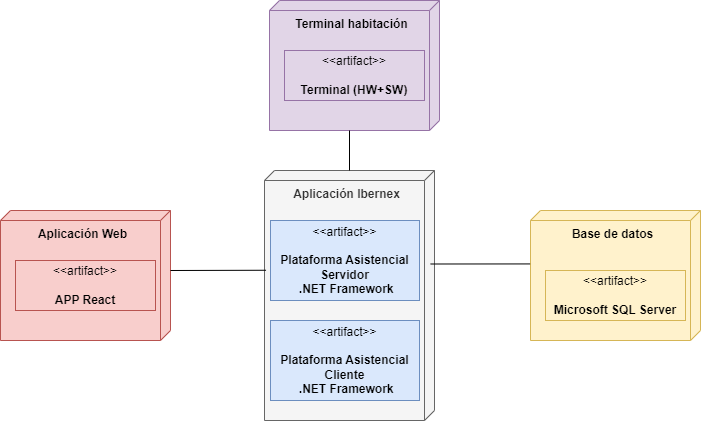
\includegraphics[width=15cm]{Imagenes/Arquitectura-despliegue}
    \caption{Diagrama de despliegue}
    \label{fig:despliegue}
\end{figure}

Con este diagrama se observan los elementos que han estado implicados en el proyecto. No obstante, lo que se ha implementado ha sido: la aplicación web completa y la funcionalidad añadida a la Plataforma Asistencial Servidor de la aplicación de Ibernex. A continuación se describen los elementos con mayor detalle:

\begin{itemize}
	\item \textbf{Plataforma Asistencial Servidor (PAServidor)} es la aplicación servidor del sistema asistencial Helpnex. Se trata de una aplicación monolítica modular. Dos de los elementos que componen la arquitectura de la aplicación son:
	\begin{itemize}
		\item Servicios: contienen la lógica del sistema Helpnex. Los servicios se cargan al inicio de la aplicación en función de la licencia adquirida. Cada servicio es el encargado de realizar una tarea específica. Algunos ejemplos de tareas son: comunicación con los terminales de habitación; gestionar las alarmas del sistema; comunicación con la aplicación web de monitorización; localización en interiores; y comunicaciones SIP, entre otras.
		\item Cola de eventos: es el mecanismo de comunicación que utilizan los servicios para transmitir información entre ellos. Cada servicio se suscribe a una serie de eventos.
	\end{itemize}
	\item La \textbf{base de datos} es la que permite realizar la persistencia de datos de PAServidor, PACliente, la institución, los pacientes y resto de datos necesarios.
	\item La \textbf{aplicación web} que recibe los datos necesarios a monitorizar desde el nuevo servicio añadido a PAServidor para mostrarlos.
	\item \textbf{Plataforma Asistencial Cliente (PACliente)} es la encargada de gestionar la información del sistema Helpnex y guardarla en la Base de Datos. Se comunica con el PAServidor mediante una conexión socket TCP. La información se utiliza por PAServidor para realizar las gestiones necesarias. De igual forma se compone de módulos que se gestionan mediante una licencia y permiten gestionar distintos elementos. Uno de los módulos sirve para configurar un sistema de reglas de notificación ante una alarma y esto es lo que permite al sistema generar las reglas y notificar por puestos la información que debe ser mostrada en la aplicación web.\\
	PACliente se ha utilizado en el proyecto  para realizar la gestión de plantas, habitaciones, residentes, terminales, trabajadadores, recursos de los puestos y configuración de reglas, teniendo una institución ficticia generada con datos de prueba durante todo el desarrollo.
	\item El \textbf{terminal} es el hardware que se encuentra en la habitación. En este contexto sirve tanto para notificar y codificar las alarmas como para registrar las presencias de trabajadores en las habitaciones. Existen otras tareas adicionales que pueden ser realizadas, pero que no están directamente relacionadas con el alcance de este proyecto.
\end{itemize}

% Hacer referencia al Anexo donde se expliquen las alternativas que se plantearon
La arquitectura aquí expuesta es la elegida entre las distintas opciones barajadas. Estas otras se pueden consultar con detalle en el \hyperref[anexo-a]{Anexo A}.\\

% Arquitectura del PAServidor
Para entender mejor la arquitectura del PAServidor se proporciona un diagrama más detallado (véase la Figura \ref{fig:PAServidor}).

\begin{figure}[H]
    \centering
    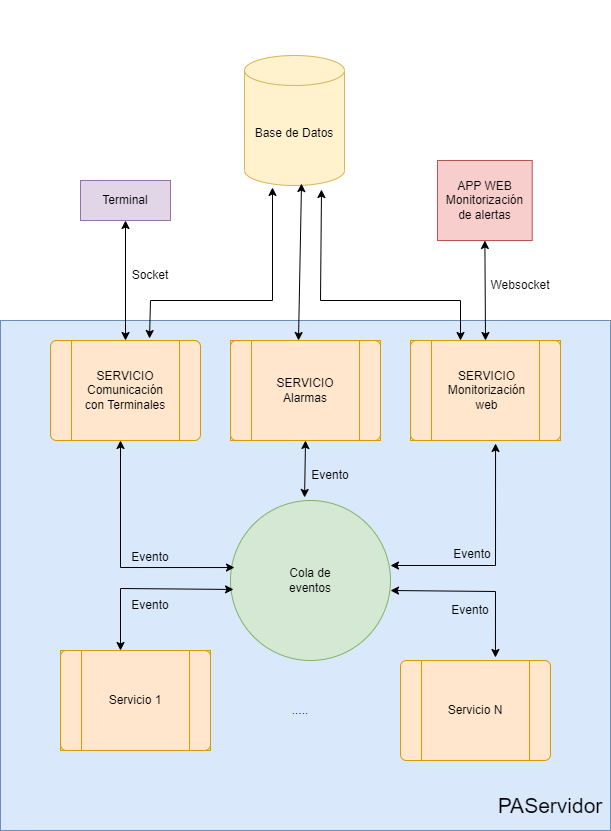
\includegraphics[width=12cm]{Imagenes/Arquitectura-PAServidor}
    \caption{Diagrama arquitectura PAServidor}
    \label{fig:PAServidor}
\end{figure}


% Explicar comportamiento de servicios y eventos
\section{Comportamiento servicios y eventos}
% TODO: DIAGRAMAS DE COMPORTAMIENTO para mostrar ejemplo/s de funcionamiento interno.
Respecto al comportamiento de los servicios y eventos implicados, a continuación se exponen uno ejemplo de funcionamiento tanto para alarma como para presencia.\\

El funcionamiento para el caso de las alarmas es el que se presenta en la Figura \ref{fig:flujograma-alarmas}.

\begin{figure}[H]
    \centering
    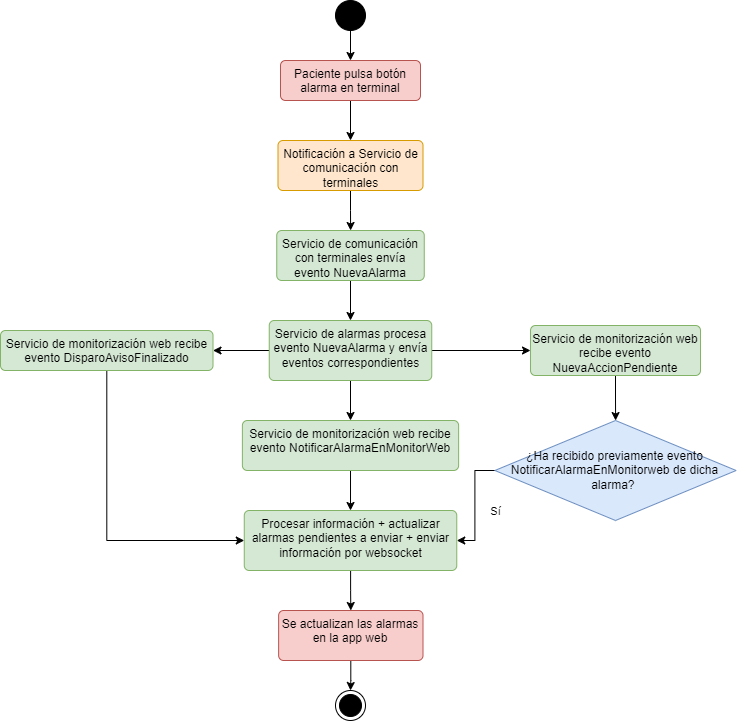
\includegraphics[width=15cm]{Imagenes/Flujograma-alarmas.png}
    \caption{Diagrama de comportamiento - Alarmas}
    \label{fig:flujograma-alarmas}
\end{figure}

Con más detalle el comportamiento es el siguiente:
\begin{enumerate}
	\item El paciente pulsa el botón del terminal para solicitar ayuda.	
	\item El terminal notifica al \textit{servicio de comunicación con terminales}, mediante el socket, que alguien ha pulsado el botón.
	\item El \textit{servicio de comunicación con terminales} envía un evento \textit{NuevaAlarma} con toda la información relativa al terminal.
	\item El \textit{servicio de alarmas}, que está suscrito al evento \textit{NuevaAlarma}, recibe el evento y lo procesa. Como resultado envía un evento \textit{NuevaAccionPendiente} y \textit{NotificarAlarmaEnMonitorWeb}.
	\item El \textit{servicio de monitorización web} en primer lugar recibe el evento \textit{NuevaAccionPendiente} al que está suscrito pero se ignora ya que aún no se ha recibido el evento \textit{NotificarAlarmaEnMonitorWeb}. Seguido se recibe el evento \textit{NotificarAlarmaEnMonitorWeb} y se procesa, enviando mediante websocket la información conveniente a la aplicación web.
	\item En la aplicación web aparece la nueva alarma. Después se efectuará una presencia en el terminal (véase el comportamiento específico para las presencias).
	\item El \textit{servicio de monitorización web} recibe un evento \textit{NuevaAccionPendiente} cuando se actualiza la alarma y lo procesa si ha llegado el evento \textit{NotificarAlarmaEnMonitorWeb} para actualizar la alarma indicada. El resultado de la actualización es enviado mediante el websocket a la aplicación web.
	\item En la aplicación web aparece la alarma actualizada y después en el terminal un trabajador codifica la alarma y elimina su presencia (véase el comportamiento específico para las presencias).
	\item El \textit{servicio de monitorización web} recibe el evento \textit{DisparoAvisoFinalizado} cuando se codifica una alarma y lo procesa si le ha llegado el evento de \textit{NotificarAlarmaEnMonitorWeb} para eliminar la alarma indicada. El resultado de la actualización de las alarmas en el sistema es enviado mediante el websocket a la aplicación web.
	\item En la aplicación web desaparece la alarma actualizada.
\end{enumerate}


\newpage
El funcionamiento para el caso de las presencias es el que se presenta en la Figura \ref{fig:flujograma-presencias}

\begin{figure}[H]
    \centering
    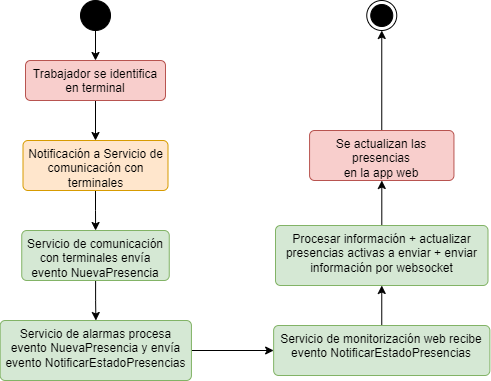
\includegraphics[width=12cm]{Imagenes/Flujograma-presencias.png}
    \caption{Diagrama de comportamiento - Presencias}
    \label{fig:flujograma-presencias}
\end{figure}

Con más detalle el comportamiento es el siguiente:
\begin{enumerate}
	\item Un trabajador se identifica en la habitación pasando su tarjeta personal por el lector o introduciendo su PIN personal.
	\item El terminal notifica al \textit{servicio de comunicación con terminales}, mediante el socket, que alguien está presente.
	\item El \textit{servicio de comunicación con terminales} envía un evento \textit{NuevaPresencia} con toda la información relativa a la presencia.
	\item El \textit{servicio de alarmas} que está suscrito al evento \textit{NuevaPresencia} recibe el evento y lo procesa. Como resultado envía un evento \textit{NotificarEstadoPresencias}.
	\item El \textit{servicio de monitorización web} recibe el evento \textit{NotificarEstadoPresencias} que puede indicar presencias actuales, la existencia de una presencia nueva, la actualización de una presencia o que una presencia ha sido eliminada, y lo procesa. Como resultado envía la información necesaria mediante el websocket a la aplicación web.
	\item En la aplicación web aparece, se actualiza o desaparece la presencia.
\end{enumerate}

\section{Base de datos}

% Explicar qué partes de la base de datos utilizo de su sistema y con diagramas

Para llevar a cabo el desarrollo, fue proporcionada por parte de la empresa una base de datos de prueba configurada siguiendo el modelo de datos existente de la aplicación de Ibernex.\\

Parte de la información que se tiene que enviar a la web se puede obtener de los eventos que se reciben en el servicio, pero para obtener otros datos es necesario acceder a la base de datos. A continuación se exponen los diagramas de la base de datos utilizados en el contexto de este proyecto. Estos diagramas han sido realizados con la aplicación Microsoft SQL Server Management Studio \cite{sql-server-studio}. \\

En la Figura \ref{fig:Diagrama-BD-Login} se presenta la parte del modelo correspondiente a los trabajadores y la información necesaria para realizar el login. El trabajador se define como un usuario del sistema de monitorización web. Se observa que la mayor parte de información personal de los trabajadores se encuentra en la tabla persona que se comparte con otras entidades de la base de datos. La tabla de imagenes proporciona la foto que identifica al trabajador.

\begin{figure}[H]
    \centering
    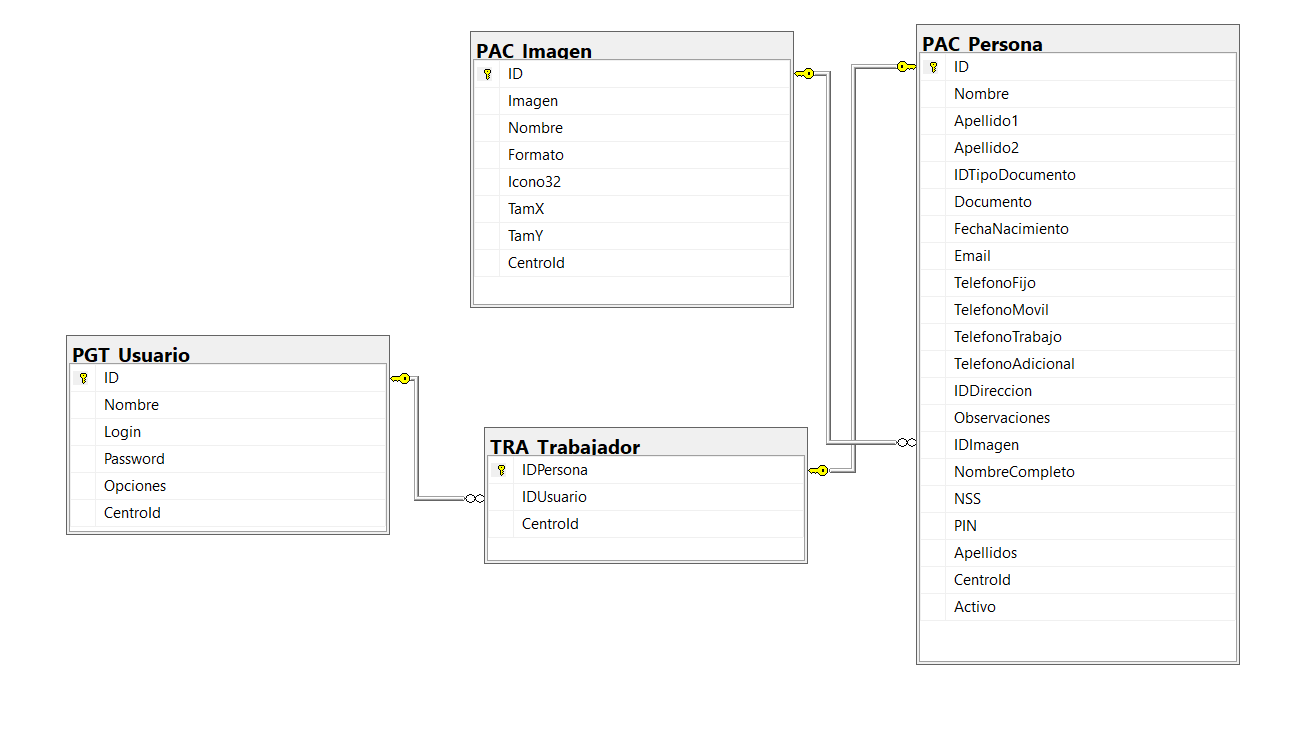
\includegraphics[width=16cm]{Imagenes/Diagrama-BD-Login}
    \caption{Diagrama base de datos - Trabajadores}
    \label{fig:Diagrama-BD-Login}
\end{figure}

\newpage
En la Figura \ref{fig:Diagrama-BD-Clientes} se presenta la parte del modelo correspondiente a los clientes, es decir, a los pacientes de la institución sanitaria. Se observa como en este modelo se encuentra tanto la información personal del paciente (en la tabla de personas de igual forma que con los trabajadores) como la información relacionada con la ubicación del paciente dentro de la institución. En este caso la tabla de imagenes proporciona la foto que identifica al paciente y en el caso de las zonas el plano de la planta en la que se encuentra el paciente.

\begin{figure}[H]
    \centering
    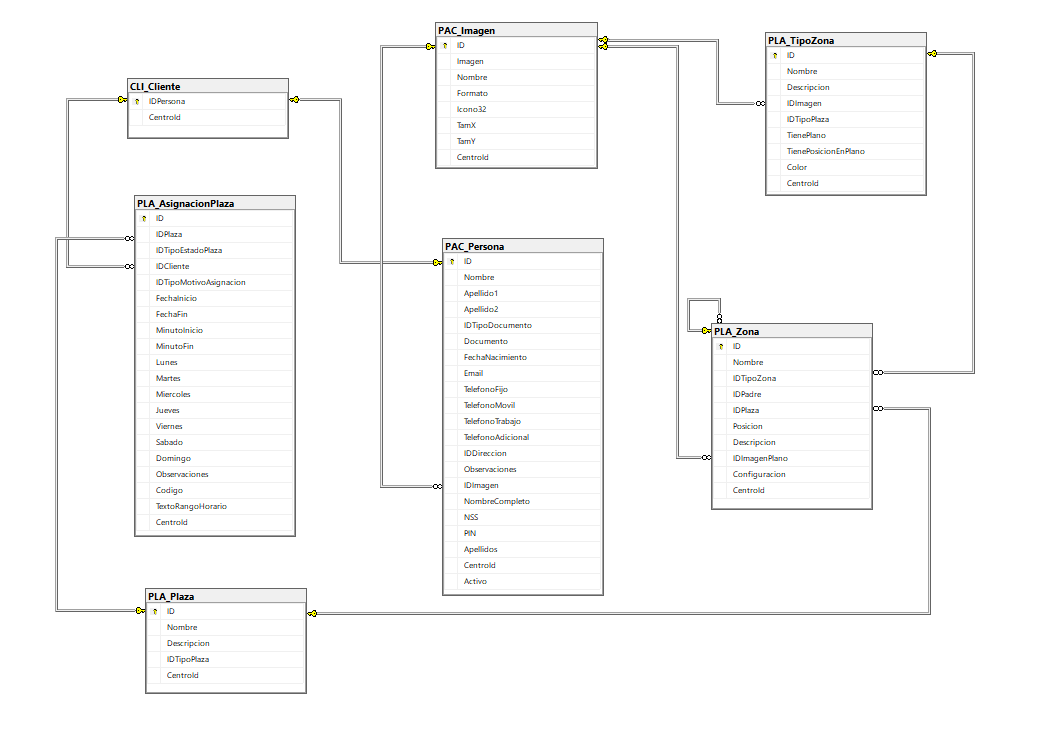
\includegraphics[width=16cm]{Imagenes/Diagrama-BD-Clientes}
    \caption{Diagrama base de datos - Clientes}
    \label{fig:Diagrama-BD-Clientes}
\end{figure}

\newpage
En la Figura \ref{fig:Diagrama-BD-Alertas} se presenta la parte del modelo en la que se encuentra toda la información de las alarmas en el sistema. De las tablas de este diagrama se obtiene la información necesaria que se debe procesar en los distintos servicios para enviar los eventos correspondientes en Helpnex. En otros casos es necesario realizar accesos a la base de datos para obtener la información que se monitoriza en la web.

\begin{figure}[H]
    \centering
    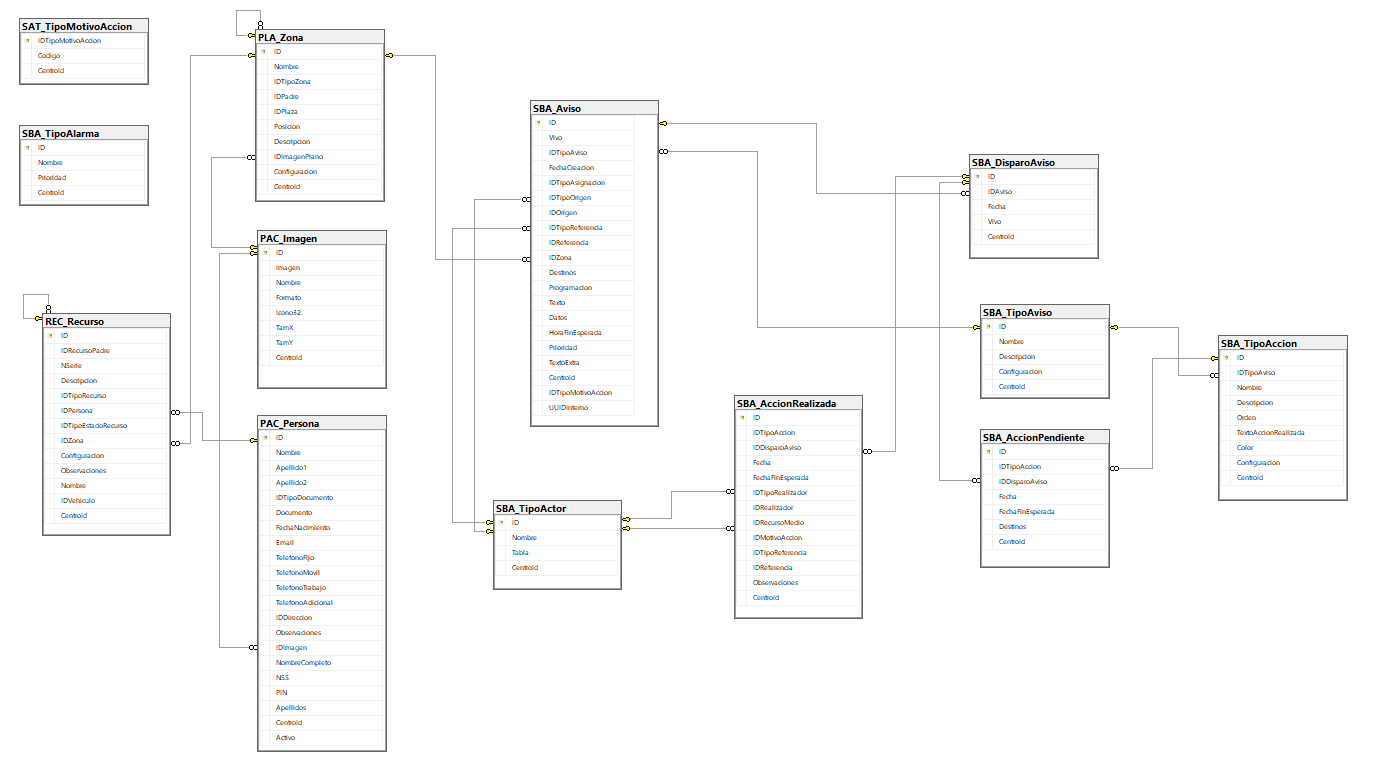
\includegraphics[width=16cm]{Imagenes/Diagrama-BD-Alertas}
    \caption{Diagrama base de datos - Alarmas}
    \label{fig:Diagrama-BD-Alertas}
\end{figure}

\newpage
En la Figura \ref{fig:Diagrama-BD-Presencias} se presenta la parte del modelo correspondiente a la información de las presencias en el sistema. En estas tablas se ve reflejada la información necesaria a procesar en los servicios para enviar la información en los eventos relacionados con las presencias o la información necesaria que hay que obtener para monitorizarla en la web si no llega en el evento recibido.

\begin{figure}[H]
    \centering
    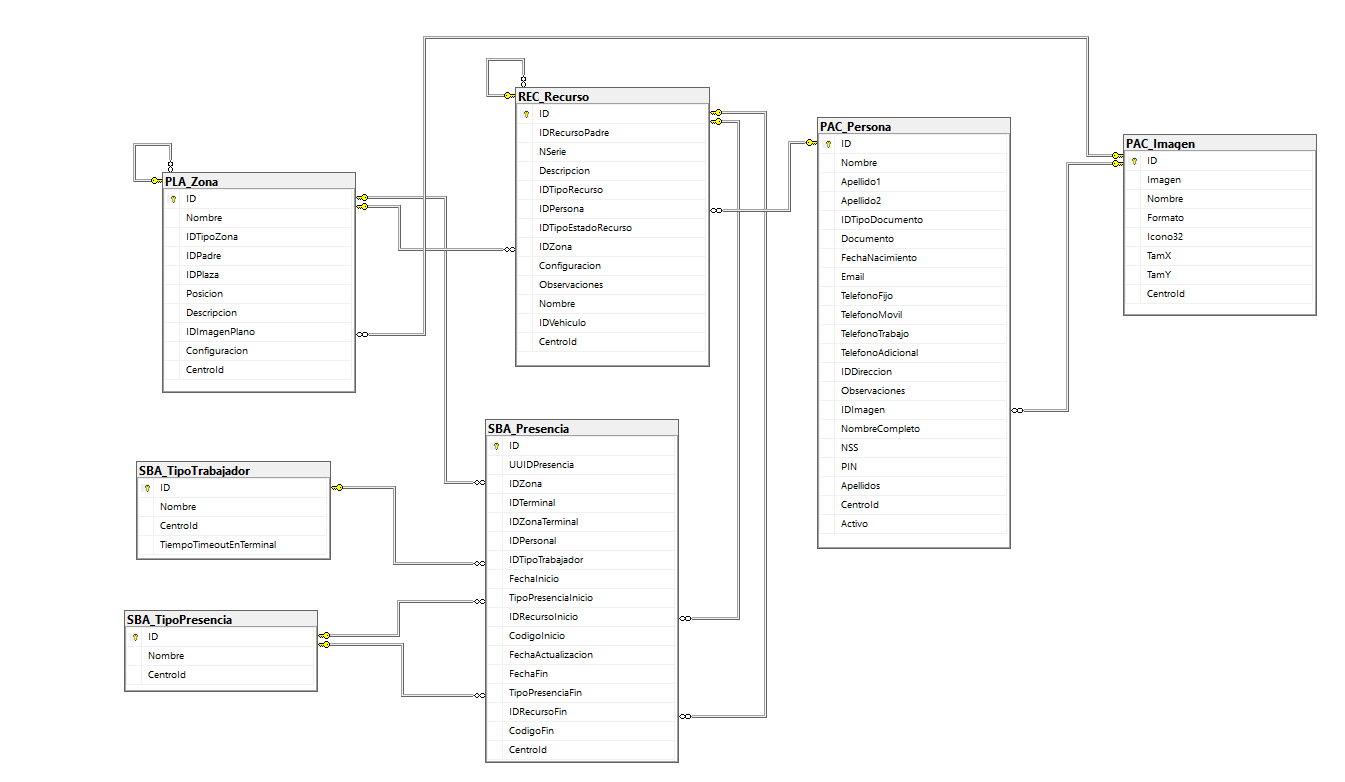
\includegraphics[width=16cm]{Imagenes/Diagrama-BD-Presencias}
    \caption{Diagrama base de datos - Presencias}
    \label{fig:Diagrama-BD-Presencias}
\end{figure}

\newpage
\section{Interfaz de usuario}
\label{section-ui}
% Poner la interfaz final del usuario cuando esté terminada

En esta sección se explica la interfaz de usuario final de la aplicación y en el \hyperref[anexo-e]{Anexo E} se puede observar más ejemplos de dicha interfaz.\\


Al iniciar la aplicación, si el navegador no tiene una sesión iniciada el sistema carga la pantalla de inicio de sesión de la Figura \ref{fig:login}. \\ 

En caso de que exista un usuario con una sesión iniciada el sistema carga como pantalla principal la de la Figura \ref{fig:map}. Esta pantalla muestra las distintas plantas existentes en la institución y la cantidad de alarmas o presencias activas en dicha planta. En la parte superior se observa el carrusel con las alertas activas en el sistema pertenecientes a la planta seleccionada. A la derecha se observa el plano de la planta seleccionada. En este plano además se muestra la información referente a la ubicación de alarmas y presencias. En cada habitación si hay alguna alerta activa se colorea el espacio y se muestra un icono de la alerta con más prioridad de las existentes en el carrusel pertenecientes a dicha habitación, coloreandola según el tipo de alerta (alarma o presencia) y su estado (en caso de ser alarma) siguiendo este orden de prioridad:
\begin{enumerate}
	\item Rojo: alerta de tipo alarma y estado disparada
	\item Amarillo: alerta de tipo alarma y estado aceptada
	\item Azul: alerta de tipo alarma y estado atendida
	\item Verde: alerta de tipo presencia
\end{enumerate}
Si se clica en el icono que aparece en la habitación se muestra una ventana emergente con la misma información que se puede encontrar en el carrusel sobre esa alerta.\\

En el menú lateral de la pantalla mencionada, si se selecciona la opción de listado de alertas, se navega a la pantalla de la Figura \ref{fig:list}. Aquí se muestra una tabla con las alarmas activas existentes y ordenadas por prioridad según la fecha y hora. Tal y como se puede observar, se presenta el tipo de alerta, fecha y hora de generación, zona y paciente. En la parte superior se muestra el número total de alarmas y presencias en todas las plantas. Desde esta pantalla se puede volver al plano de alertas seleccionando la opción del menú lateral correspondiente.


\newpage

\begin{landscape}
\begin{figure}[!ht]
	\centering
	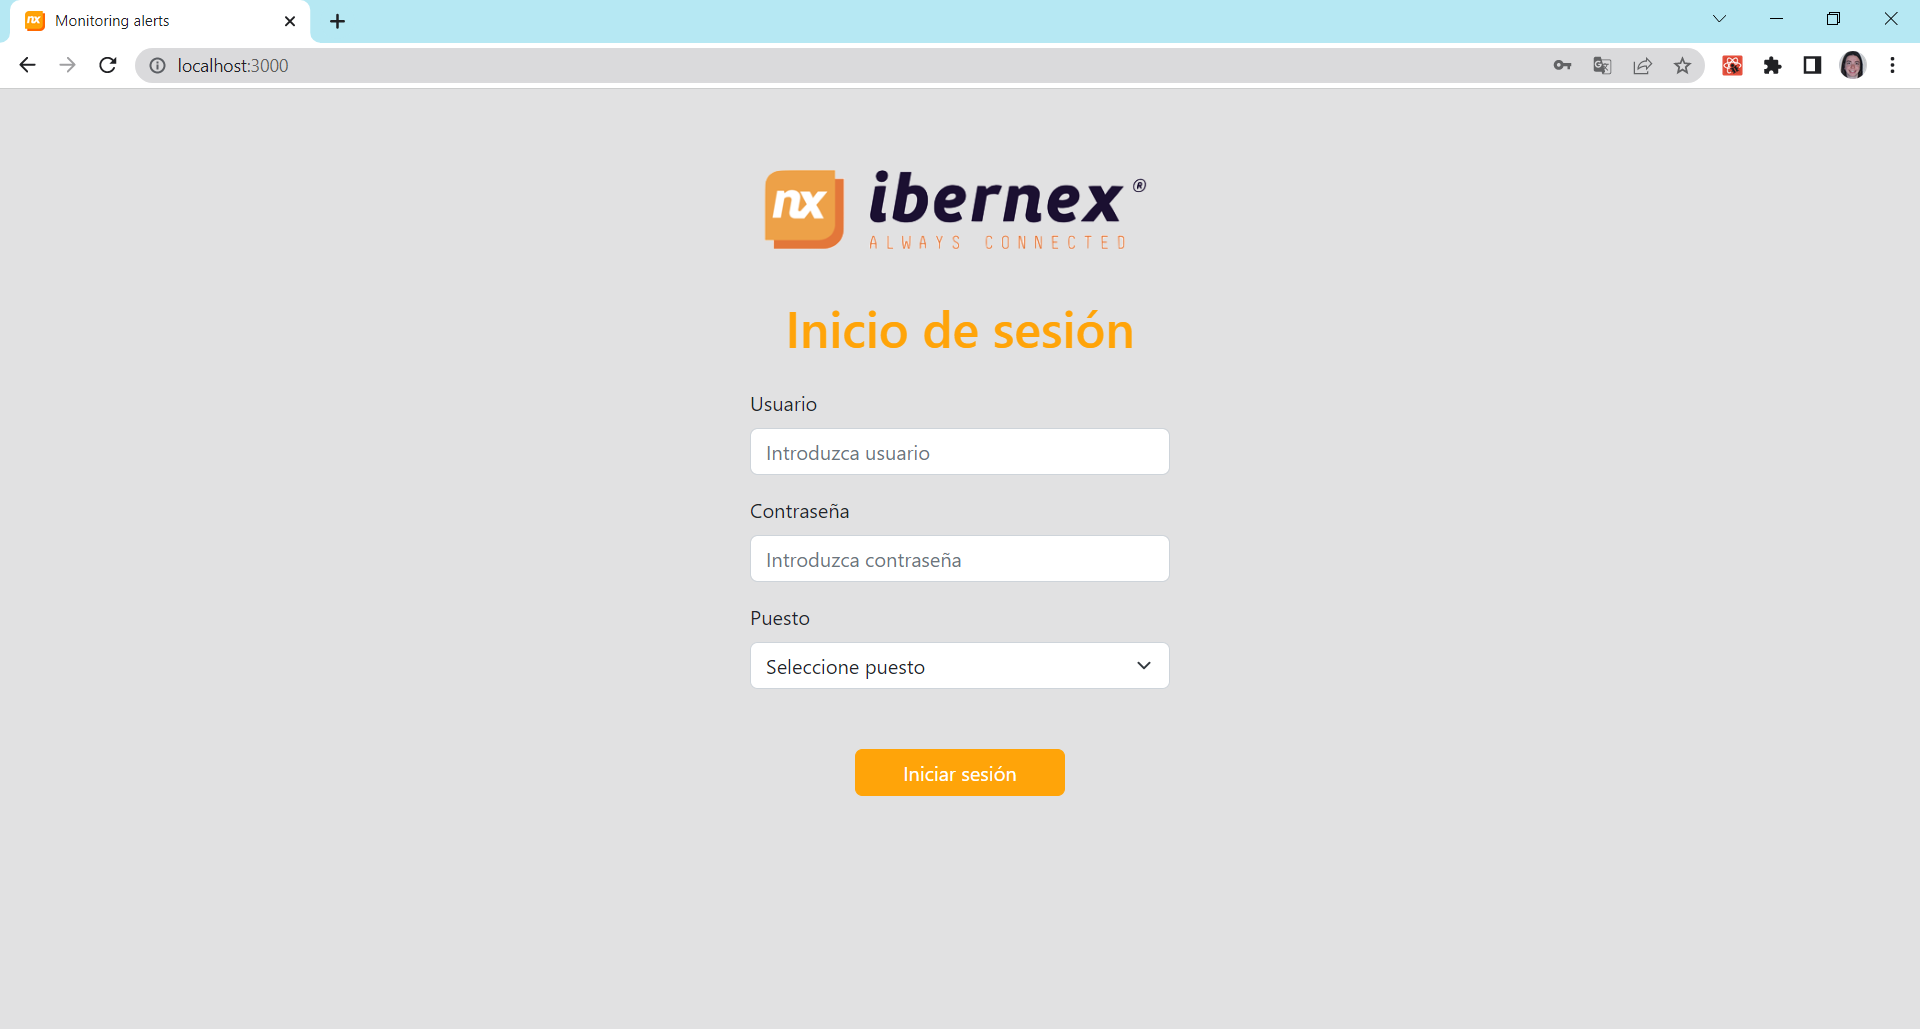
\includegraphics[width=25cm]{Imagenes/login.PNG}
	\caption{Pantalla de inicio de sesión}
	\label{fig:login}
\end{figure}

\begin{figure}[!ht]
	\centering
	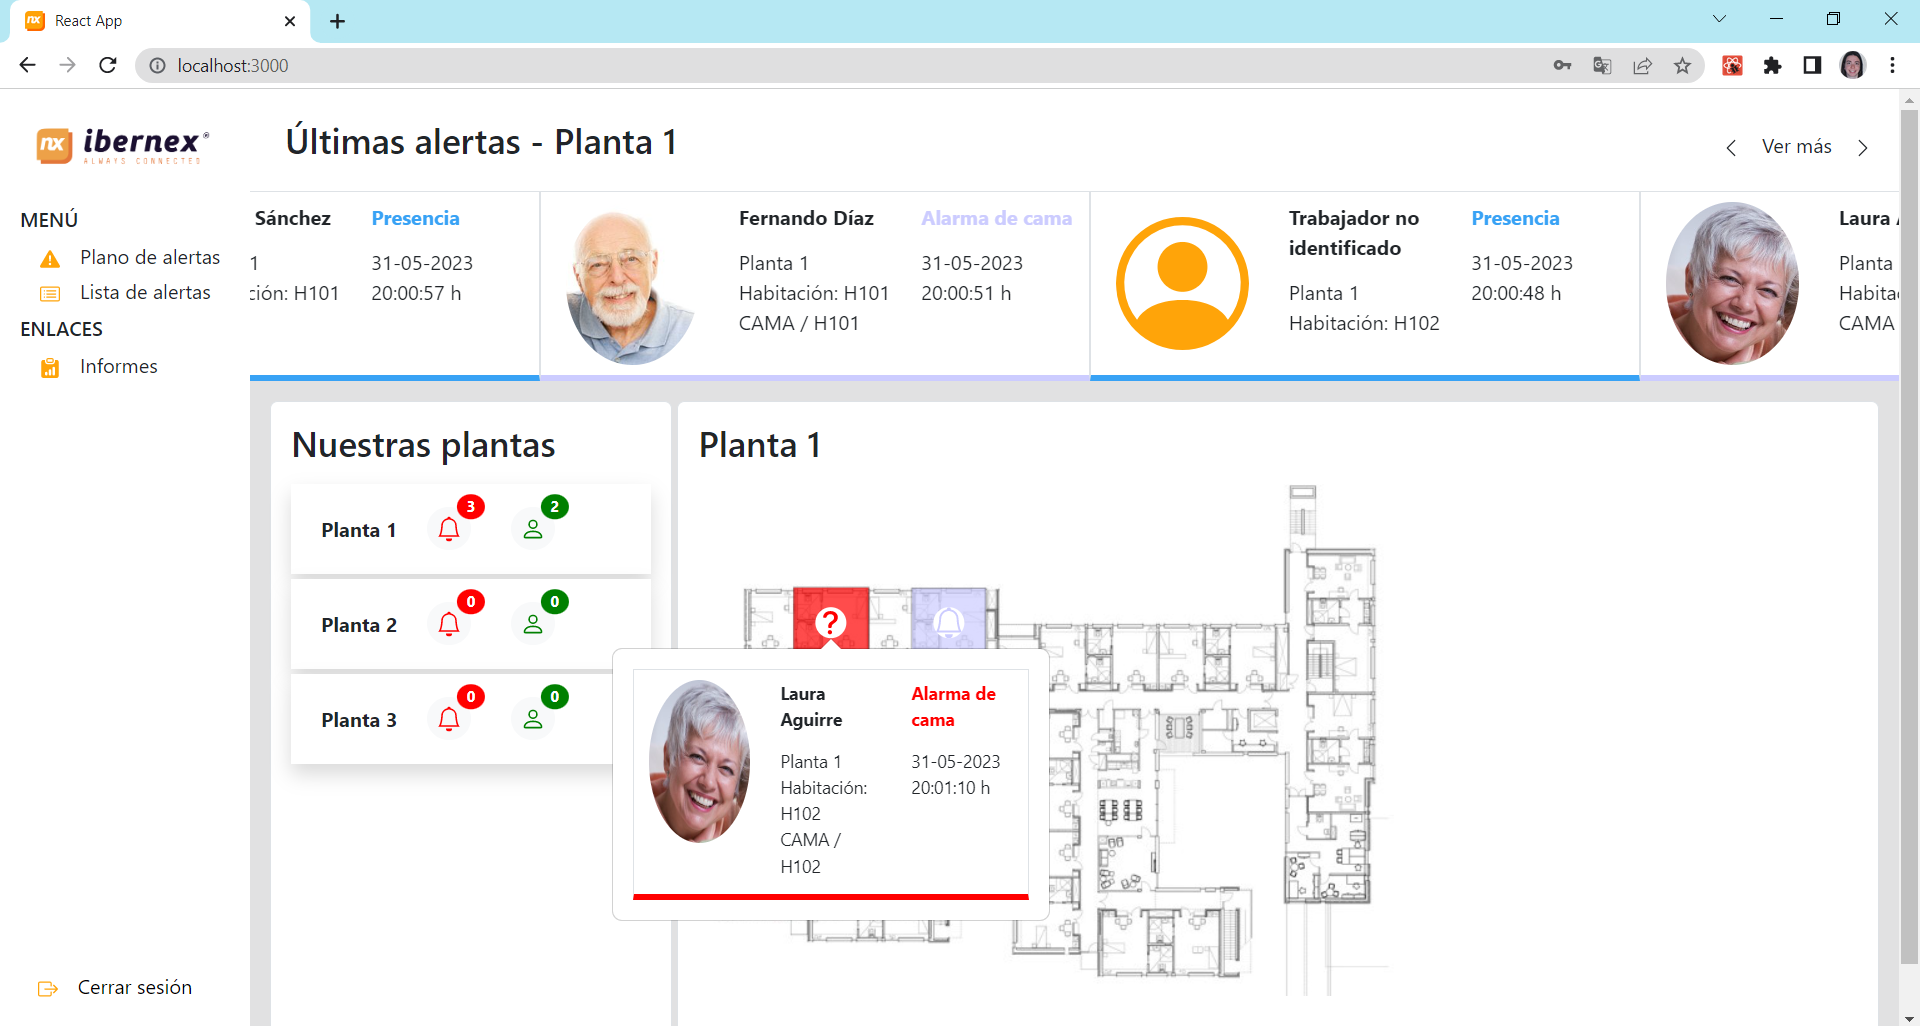
\includegraphics[width=25cm]{Imagenes/map-alarmas-estados.PNG}
	\caption{Pantalla de plano de alertas}
	\label{fig:map}
\end{figure}

\begin{figure}[!ht]
	\centering
	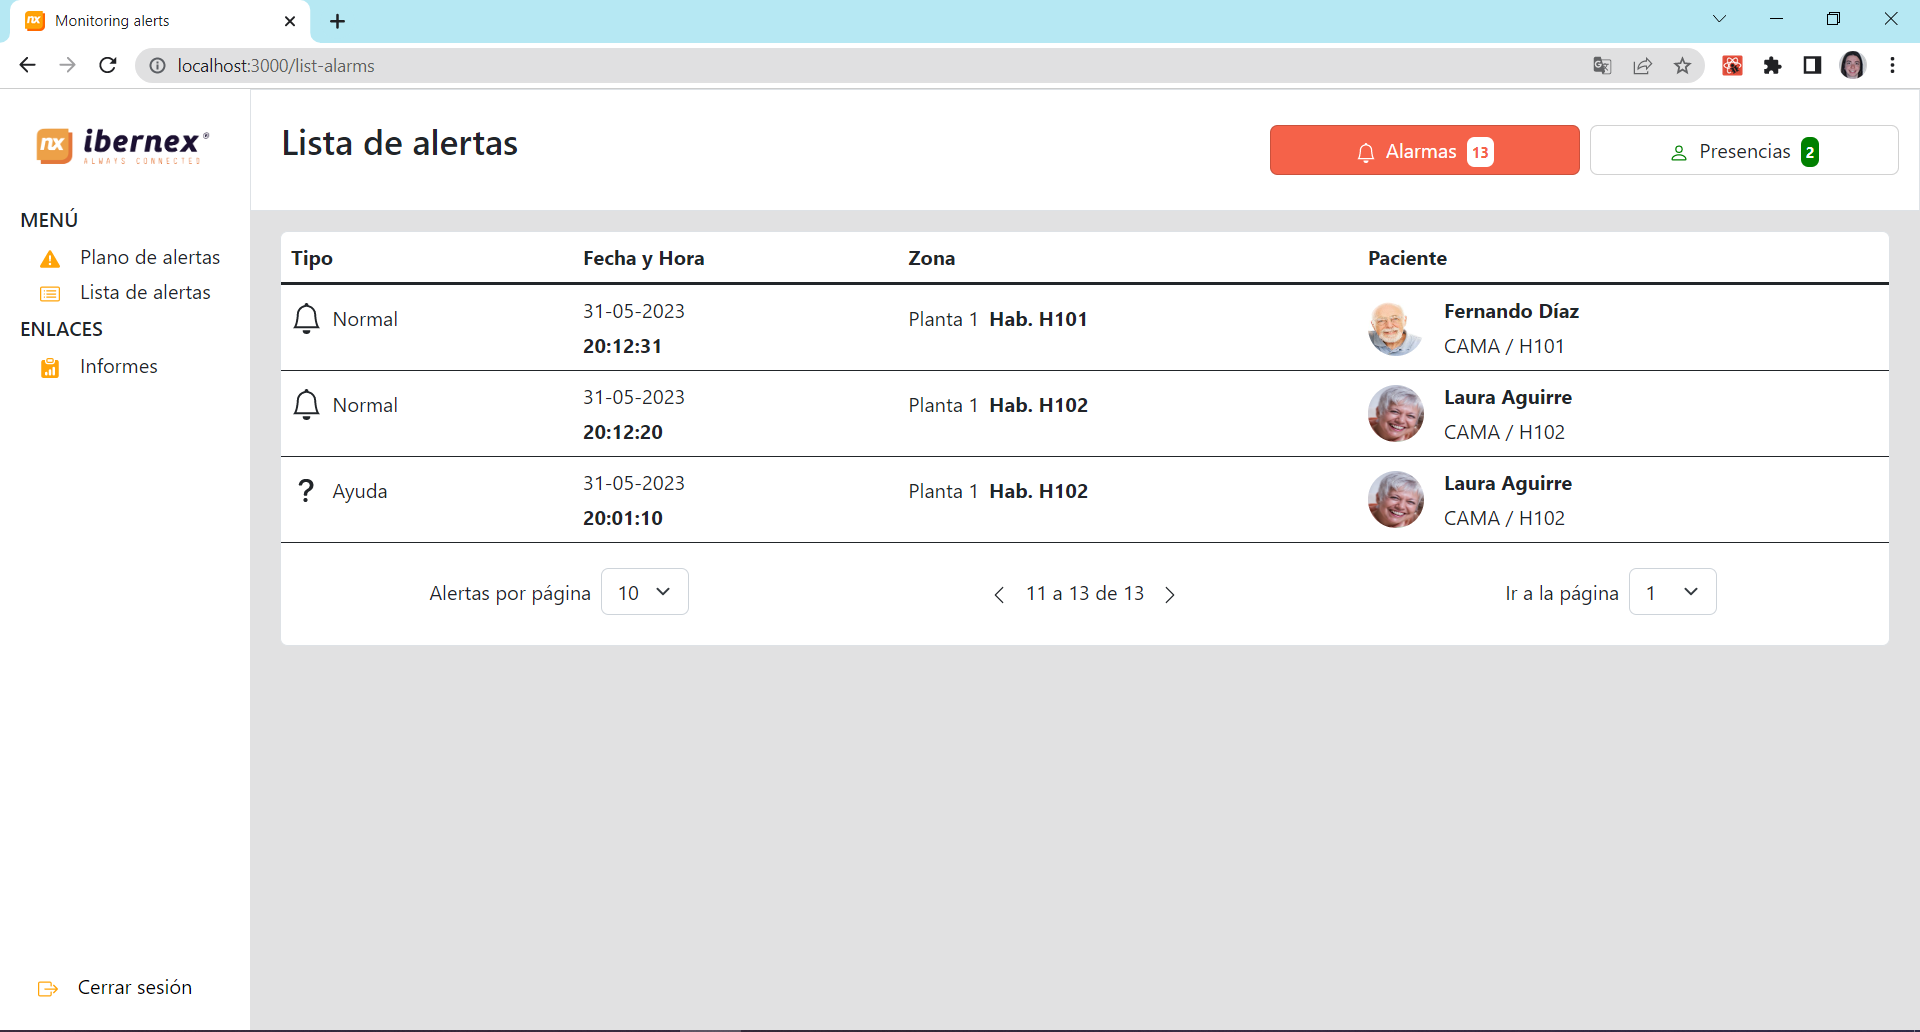
\includegraphics[width=25cm]{Imagenes/list-pag2.PNG}
	\caption{Pantalla de lista de alertas}
	\label{fig:list}
\end{figure}
\end{landscape}



